\begin{tiny}
\begin{minipage}{0.5\linewidth}
    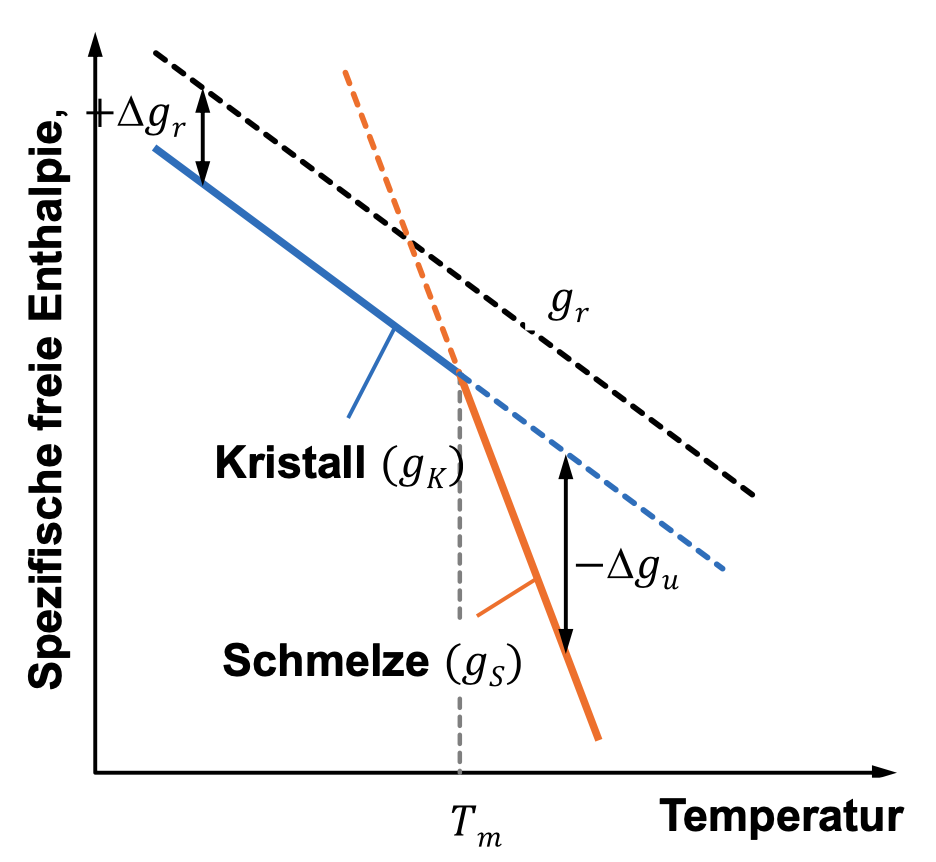
\includegraphics[width = 35mm]{src/images/Thermo_Erstarrung.png}

\end{minipage}
\begin{minipage}{0.5\linewidth}
    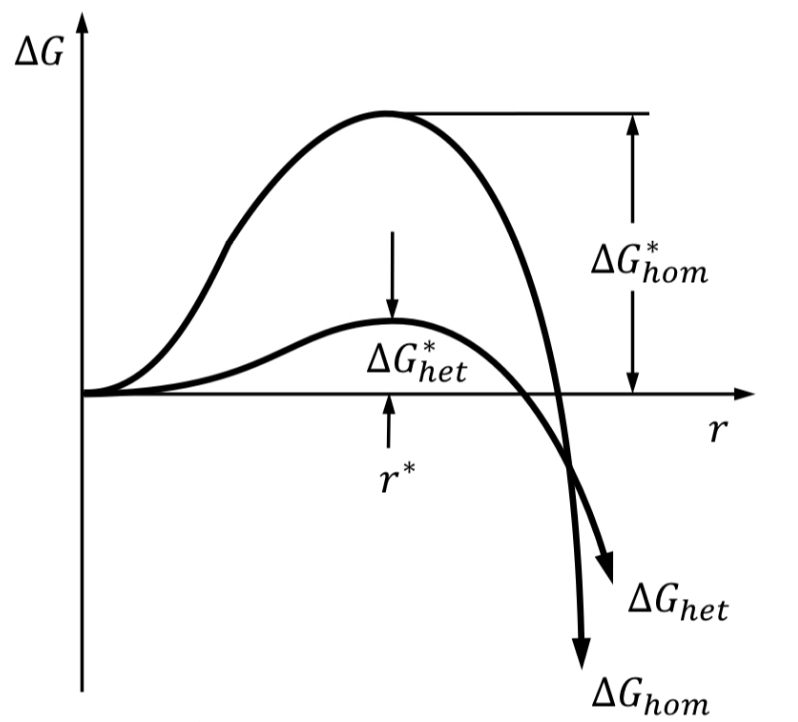
\includegraphics[width = 35mm]{src/images/Embryo_vs_Keim.png}

\end{minipage}

\begin{minipage}{0.5\linewidth}
    Unterkühlung: 
    $ \Delta g_u = g_s - g_K$\\
\end{minipage}
\begin{minipage}{0.5\linewidth}

    
    \begin{center}
        \begin{align*}
            \Delta G_u(r) &= - \frac{4}{3}\pi r^3\Delta g_u\\
            \Delta G_G(r) &= 4\pi r^2 \sigma
        \end{align*}
    \end{center}
\end{minipage}
\vspace{2mm}


\begin{minipage}{0.55\linewidth}
    Ein Keim kann nur dann wachsen wenn die \\
    freiwerdendende Umwandlungsenergie $\Delta G_u(r)$ grösser ist als die Grenzflächenenergie $\Delta G_G(r)$
\end{minipage}
\begin{minipage}{0.45\linewidth}
    \begin{center}
        $\left| \frac{d \Delta G_u(r)}{dr} \right| > \left| \frac{d \Delta G_G(r)}{dr} \right|$\\  
    \end{center}
\end{minipage}
\vspace{1mm}
\end{tiny}

\begin{minipage}{0.6\linewidth}
    \textbf{Kritischer Radius:} Min. Radius damit Keim wächst
\end{minipage}
\begin{minipage}{0.4\linewidth}
    \[
        \boxed{       
            \begin{aligned}
                r^{*} &= \frac{2\sigma}{\Delta g_u}
            \end{aligned}
        }
    \]
\end{minipage}

\vspace{1mm}

\begin{minipage}{0.6\linewidth}
    \textbf{Dentritenarmabstand:}
\end{minipage}
\begin{minipage}{0.4\linewidth}
    \[
        \boxed{       
            \begin{aligned}
                DAS &= A \cdot t^{\frac{1}{3}}_{E}
            \end{aligned}
        }
    \]
\end{minipage}
\vspace{1mm}

Falls Abkühlrate $\uparrow $ :  lokale Erstarrungszeit $\downarrow $ und DAS $\downarrow $\\


